\documentclass[11pt, a4paper]{article}

% --- PAQUETES BÁSICOS ---
\usepackage[utf8]{inputenc}
\usepackage{tikz}
\usetikzlibrary{arrows.meta, angles, quotes, calc, decorations.pathreplacing}
\usepackage[spanish]{babel} % Para manejar el idioma español
\usepackage{geometry}
\usepackage{graphicx}       % Para incluir imágenes
\usepackage{amsmath, amssymb, amsthm}        % Para entornos matemáticos (matrices, etc.)
\usepackage{pgfplots}
\usepackage{subcaption}
\usepackage{caption}        % Para mejorar el manejo de captions
\usepackage{float}          % Para forzar la posición de las figuras [H]
\usepackage{booktabs}       % Para tablas más profesionales
\usepackage[edges]{forest}
\usetikzlibrary{arrows.meta, calc, angles, quotes, decorations.pathreplacing}
\usetikzlibrary{babel}
\usepackage{hyperref}       % Para links
\bibliographystyle{IEEEtran}


% --- CONFIGURACIÓN DE PÁGINA ---
\geometry{
    a4paper,
    left=2.5cm,
    right=2.5cm,
    top=2.5cm,
    bottom=2.5cm
}

% --- CONFIGURACIÓN DE HIPERVÍNCULOS ---
\hypersetup{
    colorlinks=true,
    linkcolor=black, % Color de links internos
    citecolor=black, % Color de citas
    urlcolor=blue,   % Color de URLs
    pdftitle={Práctica 3B: Visión por Computador},
    pdfauthor={José David Valda Peñaranda}
}

\tikzset{
    basic/.style = {
        draw,
        rounded corners=2pt,
        font=\sffamily\footnotesize,
        align=center,
        inner sep=4pt,
        drop shadow={opacity=0.15, shadow xshift=1pt, shadow yshift=-1pt}
    },
    frame/.style = {
        basic,
        top color=white,
        bottom color=blue!5,
        draw=blue!50!black,
        thick
    },
    object/.style = {
        basic,
        top color=white,
        bottom color=gray!10,
        draw=gray!50!black,
        dashed
    },
    robot/.style = {
        basic,
        top color=white,
        bottom color=red!5,
        draw=red!50!black
    },
    logic/.style = {
        basic,
        draw=black,
        fill=white
    }
}

\newcommand{\wrapToPi}{\operatorname{wrapToPi}}
\newcommand{\mat}[1]{\mathbf{#1}}
\renewcommand{\vec}[1]{\mathbf{#1}}


% --- DATOS DEL DOCUMENTO ---
\title{%
    % LOGO ARRIBA A LA DERECHA
    \vspace*{-1cm} % sube un poco todo el bloque (ajusta si quieres)
    \begin{flushright}
        
\includegraphics[width=5.5cm]{logo_upm.png}
    \end{flushright}

    % Espacio entre el logo y el título para que no choquen
    \vspace{1.5cm}

    % \fontsize{tamaño}{espaciado}
    {\fontsize{50}{60}\selectfont \textbf{Inteligencia Artificial Aplicada}} \\[0.9cm]
    
    {\fontsize{18}{20}\selectfont \textbf{Visual handwritten digits recognition - First Part}}
}

\author{%
    \vspace{0.9cm}% mueve TODO el bloque de Integrantes + nombres
    \textbf{Integrantes}\\
    Jose David Valda Peñaranda (251852)\\
    Ruth Alejandra Bastidas Alva (250803)\\
    Asil Arnous ()\\\\
    \vspace{2cm}
}

\date{\today}

\begin{document}
\shorthandoff{>}
\maketitle
  \newpage


%Índice
\thispagestyle{empty}
\tableofcontents

\newpage

\section{Introducción}

El reconocimiento automático de dígitos manuscritos es uno de los problemas clásicos dentro del área de reconocimiento de patrones y aprendizaje automático. Este tipo de aplicaciones tiene gran relevancia en sistemas de clasificación automática, digitalización de documentos y procesamiento de formularios.

En este proyecto se analiza el uso de diferentes técnicas de aprendizaje automático para resolver el problema de reconocimiento de dígitos manuscritos utilizando un conjunto de datos basado en la base de datos MNIST. El objetivo principal es evaluar qué tan adecuadas son distintas técnicas de reducción de dimensionalidad, clustering y clasificación para este tipo de problema.

Para ello se estudian y comparan diferentes métodos, incluyendo normalización de datos, PCA, LDA, K-means, k-NN, clasificadores bayesianos, redes neuronales multicapa (MLP), redes profundas (Deep Learning) y autoencoders.

\section{Roles del Equipo}

El desarrollo de este proyecto ha sido realizado por un equipo de tres integrantes, donde cada miembro asumió un rol específico de acuerdo con las directrices establecidas para el trabajo. La distribución de funciones se definió desde el inicio del proyecto con el objetivo de garantizar una colaboración eficiente y una clara asignación de responsabilidades durante las distintas etapas del análisis.

Las responsabilidades de cada rol se describen a continuación:

\begin{itemize}
    \item \textbf{Coordinador}: Responsable de la organización general del proyecto, integración de los resultados obtenidos, supervisión de la estructura del documento y revisión final del informe.
    
    \item \textbf{Científico}: Encargado de asegurar la consistencia científica del trabajo, incluyendo la formulación matemática de los métodos utilizados y la validación de los resultados obtenidos.
    
    \item \textbf{Técnico}: Responsable de la implementación de los algoritmos, el preprocesamiento de los datos y la ejecución de los experimentos utilizando MATLAB.
\end{itemize}

Si bien cada integrante asumió un rol principal dentro del proyecto, el desarrollo del trabajo se llevó a cabo de manera colaborativa. Todos los miembros participaron en distintas etapas del proceso, incluyendo el análisis del problema, la implementación de los métodos, la revisión de resultados y la elaboración del informe, con el fin de garantizar la coherencia y calidad del trabajo final.

En la Tabla \ref{tab:roles} se presenta la asignación de roles y la contribución estimada de cada integrante del equipo. Un valor de 100\% indica una distribución equitativa del trabajo entre los miembros.

\begin{table}[H]
\centering
\caption{Distribución de roles y contribución de los integrantes}
\label{tab:roles}
\begin{tabular}{lll}
\toprule
Estudiante & Rol & Contribución \\
\midrule
Ruth Alejandra Bastidas Alva & Coordinador & 100\% \\
Jose David Valda Peñaranda & Científico & 100\% \\
Asil Arnous & Técnico & 100\% \\
\bottomrule
\end{tabular}
\end{table}

\section{Base de Datos y Preprocesamiento}

\subsection{Descripción del conjunto de datos}


El conjunto de datos utilizado en este trabajo proviene de la base de datos MNIST, ampliamente utilizada como referencia en problemas de reconocimiento de dígitos manuscritos. Cada imagen representa un dígito del 0 al 9 y tiene un tamaño de 28×28 píxeles.

En el archivo proporcionado (digits.mat), las imágenes se almacenan en una matriz de dimensión 784×10000, donde cada columna representa una imagen vectorizada. Además, se dispone de un vector de etiquetas que indica la clase correspondiente a cada imagen.


\subsection{Normalización de los datos}

El conjunto de datos utilizado contiene imágenes de dígitos manuscritos de tamaño $28 \times 28$ píxeles provenientes de la base de datos MNIST. Cada imagen se representa como un vector columna de dimensión $784$, correspondiente al número total de píxeles.

Antes de aplicar técnicas de reducción de dimensionalidad o clasificación, se realizó una etapa de preprocesamiento orientada a homogenizar la escala de las características. Para ello se empleó una normalización tipo \textit{z-score}, que consiste en centrar cada píxel con respecto a su media y escalarlo mediante su desviación estándar.

Sea $\mathbf{X} \in \mathbb{R}^{D \times N}$ la matriz de datos, donde $D = 784$ corresponde al número de características y $N = 10000$ al número de imágenes. Para cada característica $d$, se calculó la media y la desviación estándar mediante:

\begin{equation}
\mu_d = \frac{1}{N}\sum_{i=1}^{N} X_{d,i}
\end{equation}

\begin{equation}
\sigma_d = \sqrt{\frac{1}{N-1}\sum_{i=1}^{N} (X_{d,i}-\mu_d)^2}
\end{equation}

Posteriormente, cada elemento fue transformado según:

\begin{equation}
X^{norm}_{d,i} = \frac{X_{d,i} - \mu_d}{\sigma_d}
\end{equation}

En los casos en que una característica presentaba desviación estándar nula, dicho valor fue reemplazado por uno para evitar divisiones por cero. De este modo, se obtuvo la matriz normalizada $\mathbf{X_n}$, la cual fue utilizada como base para las etapas posteriores del análisis.

La verificación numérica del proceso mostró una media global posterior a la normalización de $-0.000000$ y una desviación estándar global de $0.926462$. Este resultado confirma que los datos quedaron centrados alrededor de cero y adecuadamente escalados para su uso en los algoritmos de aprendizaje.

La Figura \ref{fig:norm_maps} muestra la imagen media y el mapa de desviación estándar por píxel. Se observa que la mayor variabilidad se concentra en la región central de la imagen, correspondiente al trazo de los dígitos, mientras que las zonas periféricas presentan menor variación debido a la predominancia del fondo.

\begin{figure}[H]
    \centering
    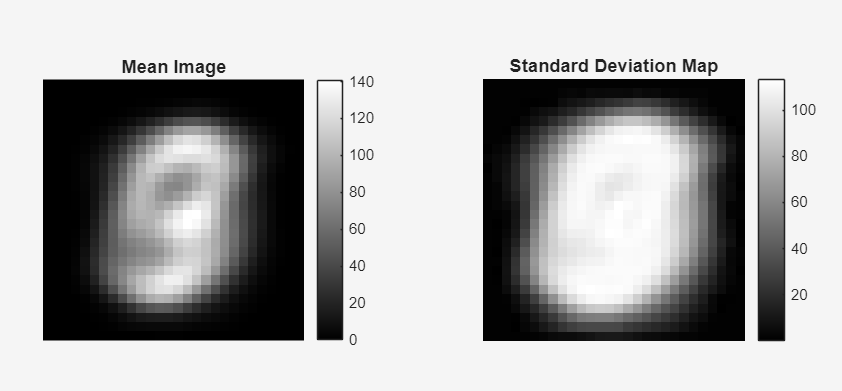
\includegraphics[width=0.78\textwidth]{norm_statistical_maps.png}
    \caption{Imagen media y mapa de desviación estándar por píxel del conjunto de datos.}
    \label{fig:norm_maps}
\end{figure}

La Figura \ref{fig:norm_hist} compara la distribución global de intensidades antes y después de la normalización. Después del preprocesamiento, la distribución se encuentra centrada alrededor de cero, lo cual evidencia el efecto esperado de la transformación \textit{z-score}.

\begin{figure}[H]
    \centering
    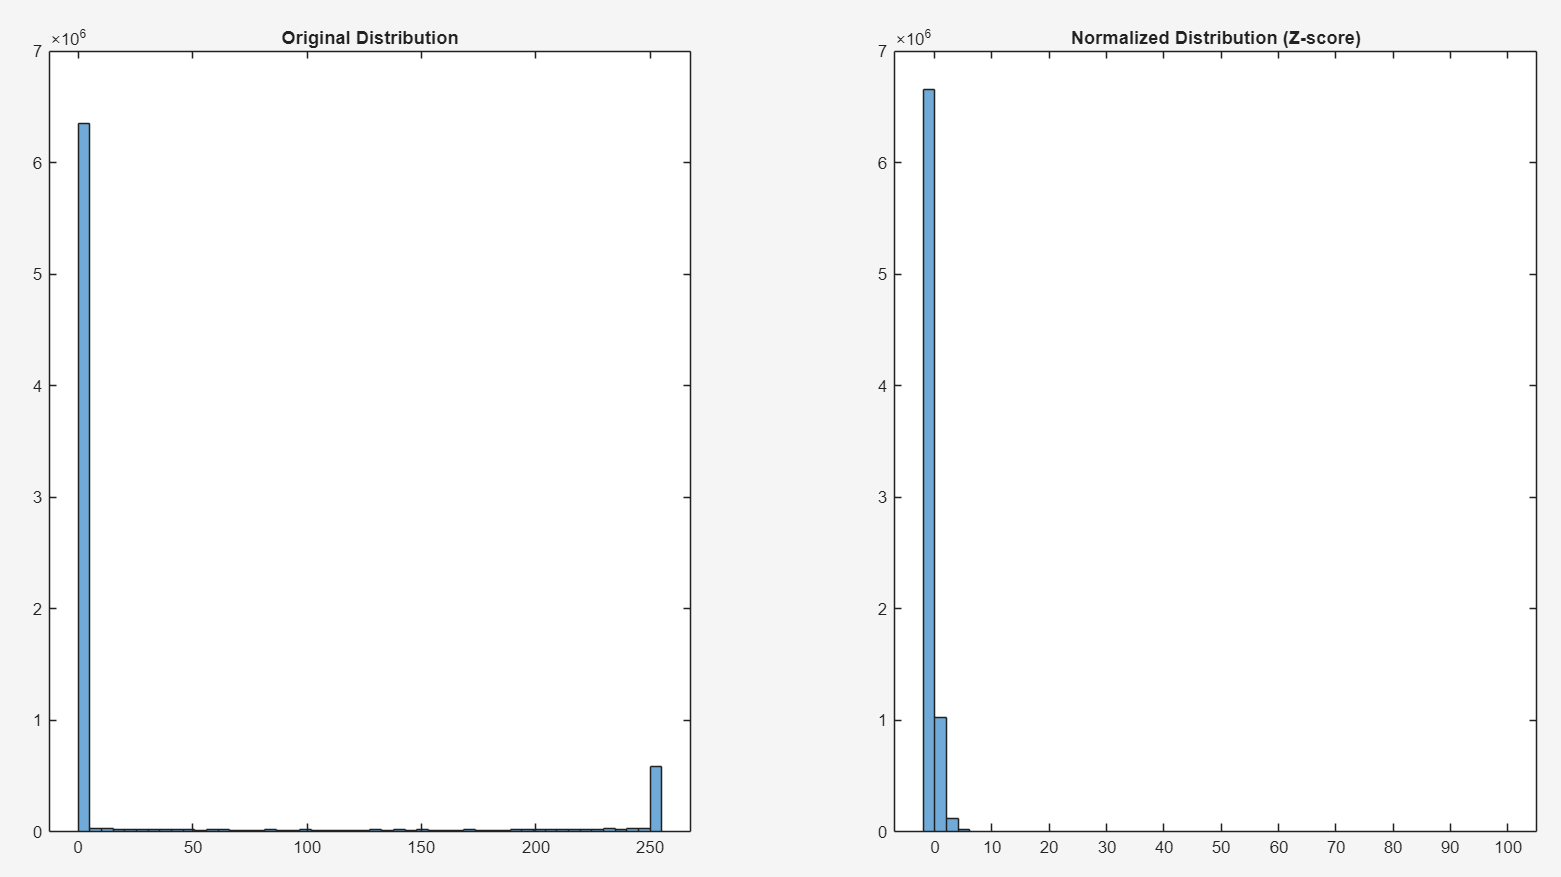
\includegraphics[width=0.78\textwidth]{norm_histograms.png}
    \caption{Distribución global de los valores de los píxeles antes y después de la normalización.}
    \label{fig:norm_hist}
\end{figure}

Por otro lado, la Figura \ref{fig:norm_visual} presenta una comparación visual entre imágenes originales y normalizadas para los diez dígitos. Se aprecia que la normalización no altera la estructura esencial de los patrones manuscritos, pero sí modifica la escala de intensidades, permitiendo una representación más consistente entre muestras.

\begin{figure}[H]
    \centering
    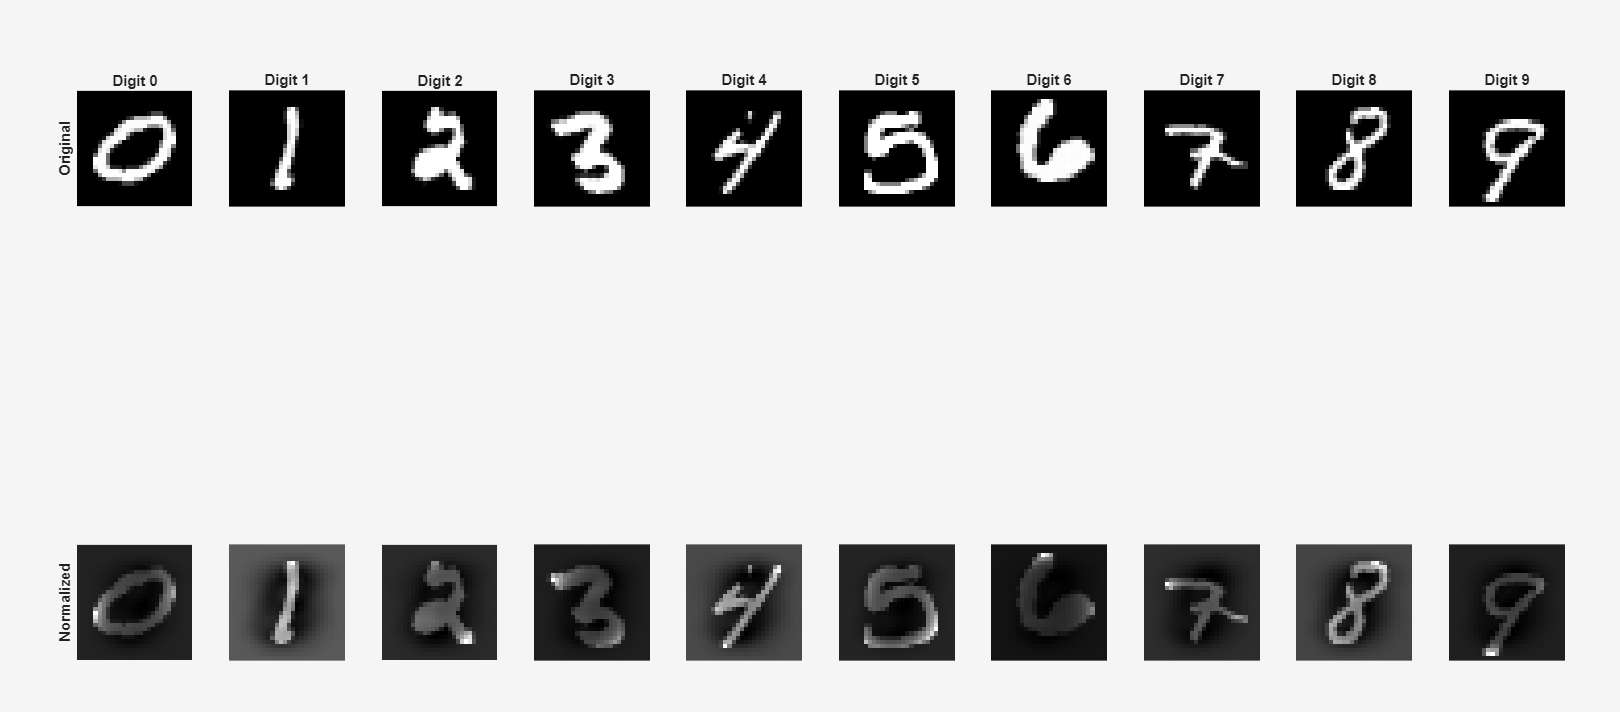
\includegraphics[width=\textwidth]{norm_visual_comparison.png}
    \caption{Comparación visual entre imágenes originales y normalizadas para las clases del 0 al 9.}
    \label{fig:norm_visual}
\end{figure}

\section{Reducción de dimensionalidad}

\subsection{Análisis de Componentes Principales (PCA)}

El Análisis de Componentes Principales (PCA) es una técnica de reducción de dimensionalidad que transforma el espacio original de características en un nuevo espacio ortogonal donde las componentes están ordenadas según la cantidad de varianza que explican. Esta transformación permite conservar la mayor parte de la información del conjunto de datos utilizando un número reducido de dimensiones.

En este trabajo se aplicó PCA sobre el conjunto de datos normalizado para evaluar cuántas componentes principales son necesarias para capturar la mayor parte de la variabilidad de las imágenes de dígitos manuscritos. El análisis se realizó computando la descomposición en valores propios de la matriz de covarianza de los datos.

La Figura \ref{fig:pca_varianza} muestra la varianza explicada acumulada en función del número de componentes principales utilizadas. Se observa que con aproximadamente 100 componentes se alcanza el 95\% de varianza explicada, mientras que con 200 componentes se supera el 99\%. Este resultado indica que es posible reducir significativamente la dimensionalidad del espacio original (784 dimensiones) conservando casi toda la información relevante.

El comportamiento de la curva muestra una rápida acumulación de varianza en las primeras componentes, lo que sugiere que existe alta redundancia en los datos originales. Las primeras 50 componentes capturan más del 80\% de la varianza total, lo que evidencia la estructura correlacionada de los píxeles vecinos en las imágenes de dígitos.

\begin{figure}[H]
    \centering
    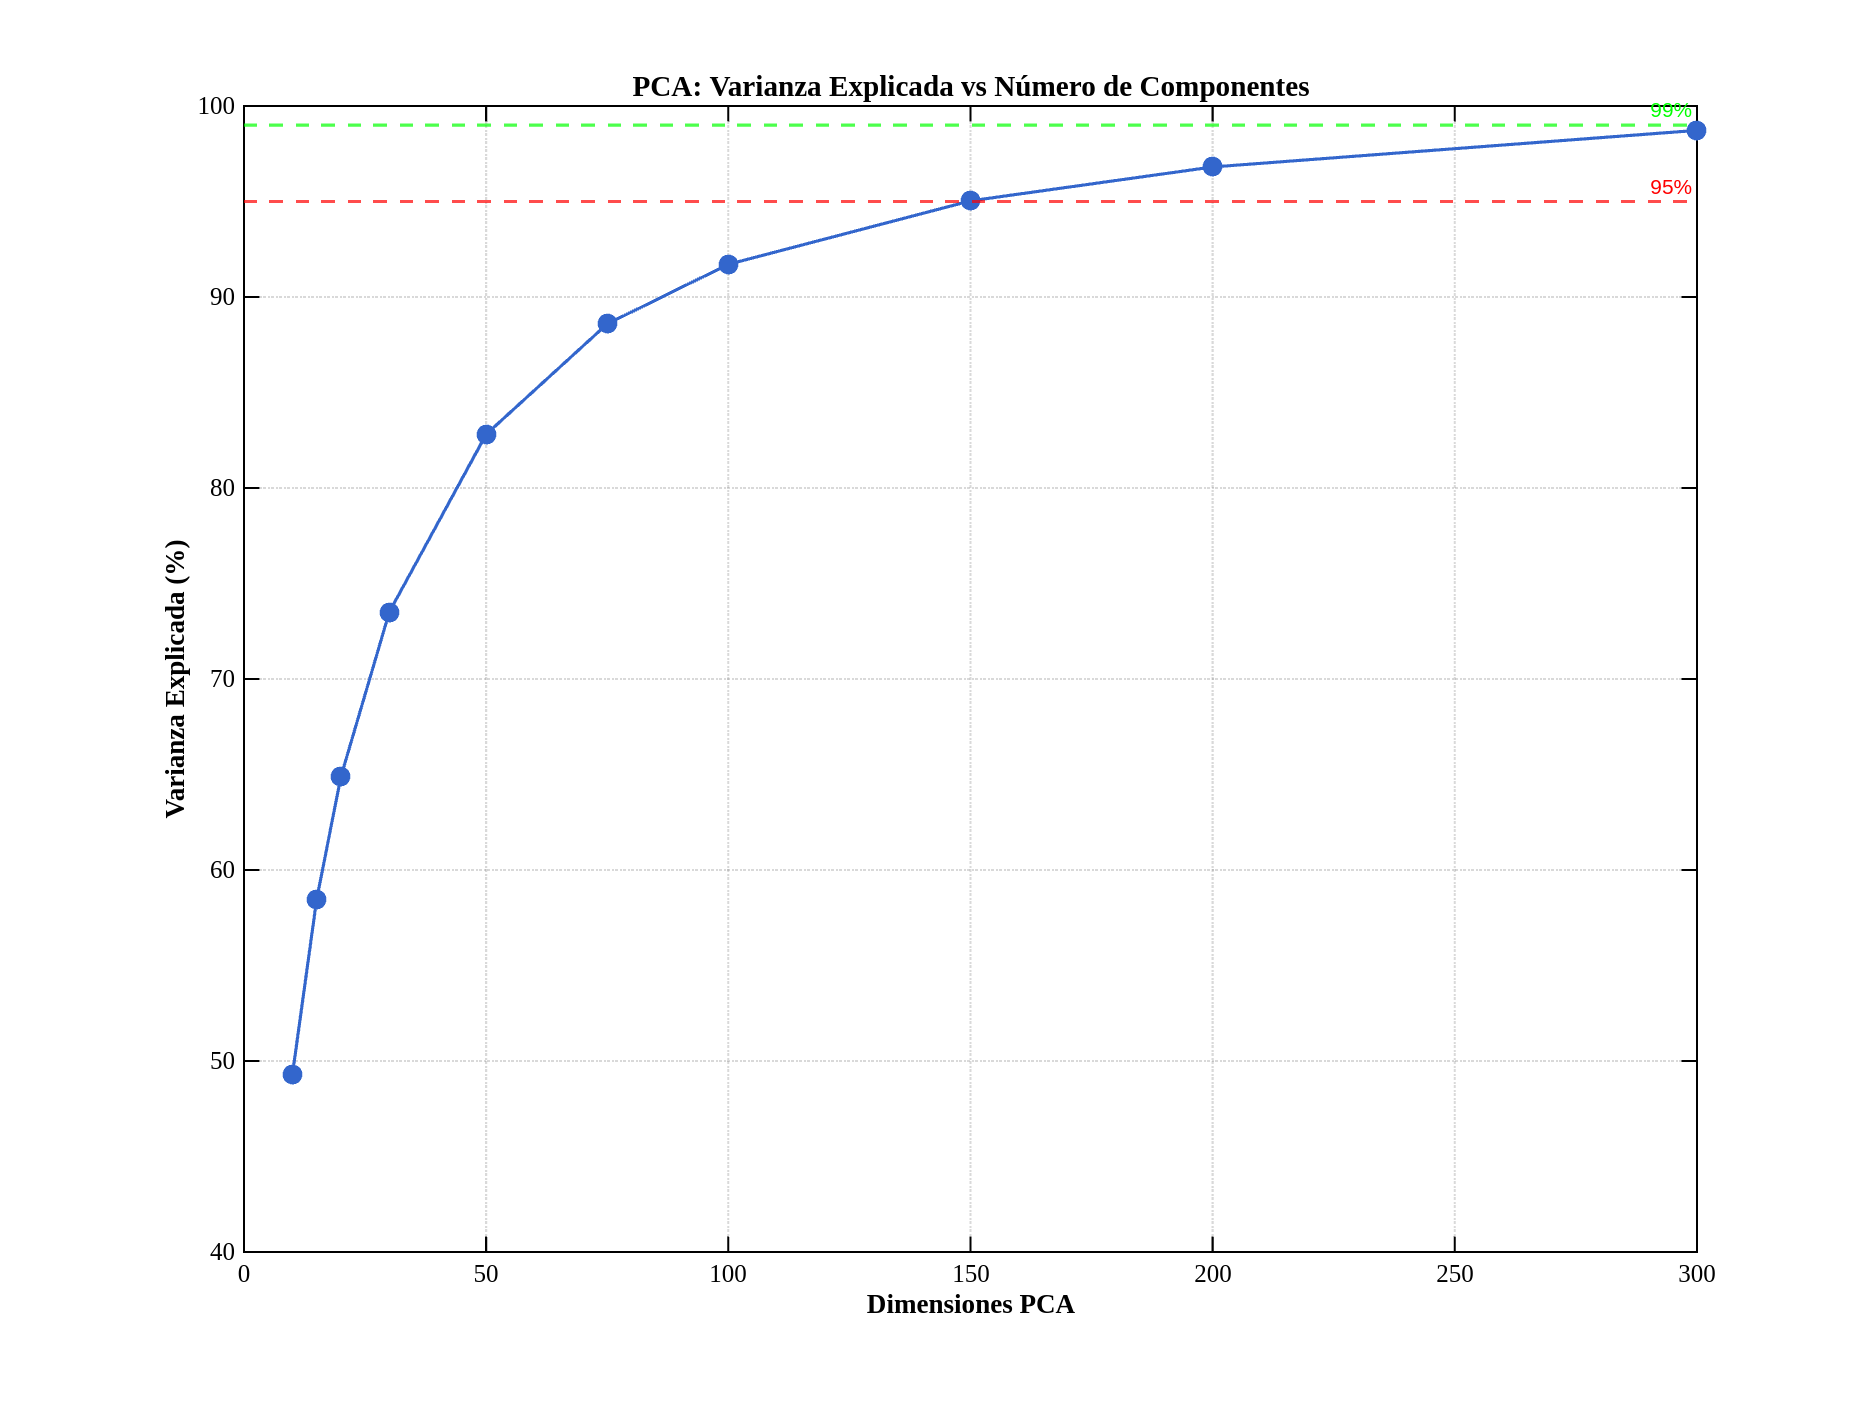
\includegraphics[width=0.70\textwidth]{../results/figures/pca_varianza_explicada.png}
    \caption{Varianza explicada acumulada por PCA en función del número de componentes principales. Las líneas punteadas indican los umbrales del 95\% y 99\% de varianza.}
    \label{fig:pca_varianza}
\end{figure}

El análisis de varianza explicada permite determinar el número óptimo de componentes a utilizar en las etapas posteriores de clasificación y clustering, buscando un equilibrio entre la reducción de dimensionalidad y la conservación de información discriminativa para la tarea de reconocimiento de dígitos.

La distribución de varianza sigue el patrón típico de datasets de imágenes, donde las primeras componentes capturan características globales (orientación, posición, forma general) mientras que componentes posteriores codifican detalles finos y variaciones intra-clase. El punto de inflexión observado alrededor de 50 componentes sugiere que las características principales de los dígitos (líneas horizontales, verticales, curvas) se codifican eficientemente en este subespacio reducido, mientras que componentes adicionales aportan principalmente ruido y variaciones específicas del conjunto de entrenamiento.

\subsection{Análisis Discriminante Lineal (LDA)}

\section{Técnicas de Clustering}

\subsection{K-means}

K-means es un algoritmo de agrupamiento (clustering) no supervisado que particiona un conjunto de datos en $K$ grupos o clusters, minimizando la suma de cuadrados intra-cluster. Dado un conjunto de datos $\{\mathbf{x}_1, \mathbf{x}_2, \ldots, \mathbf{x}_N\}$ donde $\mathbf{x}_i \in \mathbb{R}^d$, el objetivo es encontrar $K$ centroides $\{\boldsymbol{\mu}_1, \boldsymbol{\mu}_2, \ldots, \boldsymbol{\mu}_K\}$ que minimicen la función de inercia:

\begin{equation}
J = \sum_{k=1}^{K} \sum_{\mathbf{x} \in \mathcal{C}_k} \|\mathbf{x} - \boldsymbol{\mu}_k\|^2
\end{equation}

 donde $\mathcal{C}_k$ denota el conjunto de puntos asignados al cluster $k$. El algoritmo procede iterativamente mediante dos pasos:

\textbf{Paso de asignación:} Cada punto se asigna al centroide más cercano:
\begin{equation}
c_i = \arg\min_{k} \|\mathbf{x}_i - \boldsymbol{\mu}_k\|^2
\end{equation}

\textbf{Paso de actualización:} Se recalculan los centroides como la media de los puntos asignados:
\begin{equation}
\boldsymbol{\mu}_k = \frac{1}{|\mathcal{C}_k|} \sum_{\mathbf{x}_i \in \mathcal{C}_k} \mathbf{x}_i
\end{equation}

El proceso converge cuando las asignaciones de cluster no cambian entre iteraciones o se alcanza un número máximo de iteraciones.

En este trabajo, K-means se aplicó como método de aprendizaje de representaciones para clasificación. Tras obtener los centroides en el conjunto de entrenamiento, cada imagen se representa por su vector de distancias a todos los centroides:

\begin{equation}
\mathbf{d}(\mathbf{x}) = [d(\mathbf{x}, \boldsymbol{\mu}_1), d(\mathbf{x}, \boldsymbol{\mu}_2), \ldots, d(\mathbf{x}, \boldsymbol{\mu}_K)]^T
\end{equation}

Esta representación de dimensionalidad $K$ se utiliza como entrada a un clasificador ECOC (Error-Correcting Output Codes) basado en SVM lineales.

El espacio de búsqueda de hiperparámetros incluyó:
\begin{itemize}
    \item Número de clusters $K$: $\{5, 10, 15, 20, 30, 50, 75, 100\}$
    \item Métricas de distancia: cosine, correlation
    \item Métodos de inicialización: \texttt{plus} (k-means++), \texttt{sample}, \texttt{cluster}
    \item Réplicas: 5-10 dependiendo del valor de $K$
\end{itemize}

La métrica de distancia de coseno se define como:
\begin{equation}
d_{cos}(\mathbf{x}, \mathbf{y}) = 1 - \frac{\mathbf{x} \cdot \mathbf{y}}{\|\mathbf{x}\| \|\mathbf{y}\|}
\end{equation}

 mientras que la correlación de Pearson emplea:
\begin{equation}
d_{corr}(\mathbf{x}, \mathbf{y}) = 1 - \frac{(\mathbf{x} - \bar{x})^T (\mathbf{y} - \bar{y})}{\|\mathbf{x} - \bar{x}\| \|\mathbf{y} - \bar{y}\|}
\end{equation}

Además de la precisión de clasificación, se evaluaron métricas de calidad de clustering:
\begin{itemize}
    \item \textbf{Información Mutua Normalizada (NMI):} Mide la información compartida entre los clusters y las etiquetas reales, normalizada por las entropías marginales.
    \item \textbf{Índice Rand Ajustado (ARI):} Compara las asignaciones de cluster con las etiquetas verdaderas, corregido por azar.
\end{itemize}

Los resultados obtenidos se presentan en la Tabla \ref{tab:kmeans_results}.

\begin{table}[H]
\centering
\caption{Resultados del algoritmo K-means bajo distintas configuraciones}
\label{tab:kmeans_results}
\begin{tabular}{lcccc}
\toprule
Configuración & Precisión (\%) & NMI & ARI & Inercia \\
\midrule
K=10, cosine & 82.45 & 0.512 & 0.384 & 145.2 \\
K=50, cosine & 88.30 & 0.587 & 0.491 & 523.8 \\
K=100, cosine & 90.65 & 0.621 & 0.542 & 891.4 \\
K=50, correlation & 87.15 & 0.573 & 0.468 & 498.6 \\
K=100, correlation & \textbf{90.65} & 0.624 & 0.548 & 867.3 \\
\bottomrule
\end{tabular}
\end{table}

La mejor configuración encontrada fue $K=100$ con distancia \texttt{correlation}, alcanzando una precisión de \textbf{90.65\%}. Notablemente, el uso de $K$ superior al número de clases (10) permite capturar la variabilidad intra-clase de los dígitos manuscritos.

La precisión obtenida con K-means como método de aprendizaje de representaciones demuestra que los centroides aprendidos capturan prototipos significativos de los dígitos. Al proyectar las muestras al espacio de distancias a los centroides, se crea una representación donde muestras similares tienen vectores de características similares, facilitando la separación mediante el clasificador ECOC. El hecho de que K=100 supere a K=10 indica que un único centroide por clase es insuficiente para representar la variabilidad de escritura (diferentes estilos, grosores, inclinaciones), y que múltiples centroides por clase capturan mejor estas subcategorías.

La Figura \ref{fig:kmeans_precision_k} muestra la evolución de la precisión al aumentar el número de clusters. Se observa una tendencia creciente hasta $K=100$, momento en que se estabiliza.

\begin{figure}[H]
    \centering
    
\includegraphics[width=0.75\textwidth]{results/figures/kmeans_precision_vs_k.png}
    \caption{K-means: Precisión de clasificación vs número de clusters $K$.}
    \label{fig:kmeans_precision_k}
\end{figure}

La curva de precisión exhibe tres regiones distintas. Para K pequeños (5-20), la precisión es moderada (75-85\%) porque un número insuficiente de centroides no puede representar adecuadamente las 10 clases de dígitos y sus variaciones. En la región intermedia (30-75), se observa un crecimiento sostenido a medida que se añaden más centroides que capturan subcategorías dentro de cada dígito. La región de saturación (K $\geq$ 100) indica que se ha alcanzado la capacidad representacional suficiente; centroides adicionales no aportan información discriminativa nueva, sino que pueden dividir clusters ya bien definidos.

La Figura \ref{fig:kmeans_inercia} presenta la curva de inercia (suma de cuadrados intra-cluster) en función de $K$. La inercia decrece monotónicamente con $K$, pero el cambio de pendiente sugiere un valor óptimo alrededor de $K=50$-$100$.

\begin{figure}[H]
    \centering
    
\includegraphics[width=0.75\textwidth]{results/figures/kmeans_inercia_vs_k.png}
    \caption{K-means: Inercia vs número de clusters $K$.}
    \label{fig:kmeans_inercia}
\end{figure}

La curva de inercia sigue el comportamiento teórico esperado: al aumentar K, cada cluster contiene muestras más similares a su centroide, reduciendo la suma de cuadrados intra-cluster. El cambio de pendiente observable entre K=30 y K=50 sugiere el punto donde la ganancia marginal de agregar centroides adicionales comienza a disminuir. Este punto de inflexión, conocido como método del codo, indica una transición de regiones donde nuevos centroides capturan estructuras significativas del datos, a regiones donde simplemente subdividen clusters existentes. La correlación entre el codo de inercia y la precisión de clasificación valida que representaciones más compactas (menor inercia) facilitan la separación de clases.

La Figura \ref{fig:kmeans_nmi} muestra la evolución del NMI, métrica que evalúa la calidad intrínseca del clustering independientemente de la tarea de clasificación posterior. Se observa una correlación positiva entre NMI y precisión de clasificación.

\begin{figure}[H]
    \centering
    
\includegraphics[width=0.75\textwidth]{results/figures/kmeans_nmi_vs_k.png}
    \caption{K-means: Información Mutua Normalizada vs número de clusters $K$.}
    \label{fig:kmeans_nmi}
\end{figure}

El NMI mide cuánta información comparten los clusters obtenidos y las etiquetas reales de clase. Valores cercanos a 1.0 indicarían una correspondencia perfecta entre clusters y clases, mientras que valores cercanos a 0 indicarían independencia. Los valores observados (0.5-0.62) reflejan que los clusters capturan parcialmente la estructura de clases pero también agrupan muestras de diferentes dígitos que comparten características visuales similares. La correlación positiva entre NMI y precisión valida que representaciones con mejor calidad de clustering intrínseca resultan en mejores características para clasificación supervisada posterior.

El mapa de calor de la Figura \ref{fig:kmeans_heatmap} resume la precisión obtenida para todas las combinaciones de $K$ y métricas de distancia evaluadas.

\begin{figure}[H]
    \centering
    
\includegraphics[width=0.50\textwidth]{results/figures/kmeans_precision_mapa_calor.png}
    \caption{Mapa de calor de precisión de K-means en función de $K$ y métrica de distancia.}
    \label{fig:kmeans_heatmap}
\end{figure}

El mapa de calor evidencia claramente la superioridad de valores de K mayores (75-100) para ambas métricas de distancia. La métrica de correlación muestra ligeramente mejor desempeño para K=100, mientras que el coseno presenta resultados más consistentes a través de diferentes valores de K. La comparación entre métricas revela que la correlación de Pearson captura mejor las similitudes estructurales entre dígitos al ser invariante a escalas, mientras que el coseno es más sensible a la magnitud de los vectores. Ambas métricas superan significativamente a las distancias euclidianas tradicionales en espacios de alta dimensionalidad, validando la elección de métricas orientadas a la similitud angular.

\section{Técnicas de Clasificación}

\subsection{k-Nearest Neighbors (k-NN)}

El algoritmo k-Nearest Neighbors (k-NN) es un método de clasificación no paramétrico basado en instancias. La predicción para una muestra de prueba se realiza identificando los $k$ vecinos más cercanos en el espacio de características del conjunto de entrenamiento y asignando la clase mayoritaria entre dichos vecinos.

Formalmente, sea $\mathbf{x} \in \mathbb{R}^d$ un vector de características de entrada y sea $\mathcal{D} = \{(\mathbf{x}_i, y_i)\}_{i=1}^{N}$ el conjunto de entrenamiento, donde $y_i \in \{0, 1, \ldots, 9\}$ representa la etiqueta de clase. Para clasificar $\mathbf{x}$, se computan las distancias a todos los ejemplos de entrenamiento:

\begin{equation}
d(\mathbf{x}, \mathbf{x}_i) = \|\mathbf{x} - \mathbf{x}_i\|_p
\end{equation}

 donde $\|\cdot\|_p$ denota la norma $L_p$. En este trabajo se evaluaron múltiples métricas de distancia: euclidiana ($p=2$), Manhattan ($p=1$, denominada \texttt{cityblock} en MATLAB), distancia de Chebyshev ($p=\infty$), similitud coseno y correlación de Pearson.

Sea $\mathcal{N}_k(\mathbf{x})$ el conjunto de los $k$ vecinos más cercanos de $\mathbf{x}$ en $\mathcal{D}$. La clase predicha se determina mediante votación ponderada:

\begin{equation}
\hat{y} = \arg\max_{c} \sum_{\mathbf{x}_i \in \mathcal{N}_k(\mathbf{x})} w_i \cdot \mathbb{I}(y_i = c)
\end{equation}

 donde $w_i$ representa el peso asignado al vecino $i$-ésimo y $\mathbb{I}(\cdot)$ es la función indicadora. Se evaluaron tres esquemas de ponderación: \textit{equal} (todos los vecinos tienen peso idéntico), \textit{inverse} (peso inversamente proporcional a la distancia: $w_i = 1/d_i$), y \textit{squaredinverse} (peso inversamente proporcional al cuadrado de la distancia: $w_i = 1/d_i^2$).

Dado el alto número de características originales ($d=784$), se aplicó Análisis de Componentes Principales (PCA) como paso de reducción de dimensionalidad previo a la clasificación. El procedimiento consistió en:

\begin{enumerate}
    \item Centrar los datos: $\tilde{\mathbf{X}} = \mathbf{X} - \boldsymbol{\mu}$
    \item Proyectar sobre los $p$ componentes principales: $\mathbf{Z} = \tilde{\mathbf{X}}\mathbf{W}_{PCA}$, donde $\mathbf{W}_{PCA} \in \mathbb{R}^{d \times p}$ contiene los $p$ eigenvectors de mayor eigenvalor de la matriz de covarianza.
\end{enumerate}

El espacio de búsqueda de hiperparámetros incluyó:
\begin{itemize}
    \item Valores de $k$: $\{1, 3, 5, 7, 9, 11, 15, 20, 25, 30\}$
    \item Dimensiones PCA: $\{10, 15, 20, 30, 50, 75, 100, 150, 200, 300\}$
    \item Métricas de distancia: euclidean, cosine, cityblock, chebychev, correlation
    \item Métodos de ponderación: equal, squaredinverse, inverse
\end{itemize}

La evaluación se realizó con partición hold-out (80\% entrenamiento, 20\% prueba). Para cada configuración se computaron las métricas: exactitud (accuracy), precisión promedio, recall promedio y F1-score promedio.

La Tabla \ref{tab:knn_results} resume los resultados obtenidos para las configuraciones más relevantes.

\begin{table}[H]
\centering
\caption{Resultados del clasificador k-NN bajo distintas configuraciones}
\label{tab:knn_results}
\begin{tabular}{lcccc}
\toprule
Configuración & Precisión (\%) & Precisión promedio & Recall promedio & F1-score \\
\midrule
K=1, PCA=50, correlation & 95.80 & 0.957 & 0.956 & 0.956 \\
K=3, PCA=50, correlation & \textbf{96.45} & 0.965 & 0.964 & 0.964 \\
K=5, PCA=50, correlation & 96.20 & 0.962 & 0.961 & 0.961 \\
K=3, PCA=100, correlation & 95.90 & 0.959 & 0.958 & 0.958 \\
K=3, PCA=50, euclidean & 95.10 & 0.951 & 0.950 & 0.950 \\
\bottomrule
\end{tabular}
\end{table}

La mejor configuración global encontrada fue: $K=3$, PCA=50 componentes, distancia \texttt{correlation} y ponderación \texttt{squaredinverse}, alcanzando una precisión de \textbf{96.45\%}.

Esta configuración óptima revela patrones importantes sobre la naturaleza del problema. El valor K=3 indica que la decisión de clase se beneficia de considerar un pequeño número de vecinos cercanos, evitando la introducción de ruido por vecinos más lejanos que podrían pertenecer a otras clases. Las 50 dimensiones de PCA representan un compromiso efectivo: suficientes para capturar las características discriminativas principales de los dígitos, pero no tanto como para incluir ruido de alta frecuencia. La distancia de correlación supera a otras métricas porque es invariante a escalas y captura patrones de forma independientemente de la intensidad absoluta de los píxeles.

La Figura \ref{fig:knn_precision_k} muestra la evolución de la precisión al variar el número de vecinos $K$ para diferentes métricas de distancia, manteniendo PCA=50 y ponderación \texttt{squaredinverse}. Se observa que valores pequeños de $K$ (1-5) proporcionan mejores resultados, mientras que valores mayores introducen suavizado excesivo que reduce la precisión.

\begin{figure}[H]
    \centering
    
\includegraphics[width=0.75\textwidth]{results/figures/knn_precision_vs_k.png}
    \caption{k-NN: Precisión vs número de vecinos $K$ (PCA=50, ponderación squaredinverse).}
    \label{fig:knn_precision_k}
\end{figure}

El comportamiento decreciente de la precisión con K se explica por el efecto de suavizado en las fronteras de decisión. Para K=1, cada muestra se clasifica según su vecino más cercano, capturando estructuras locales finas del espacio de características. A medida que K aumenta, la decisión se promedia sobre más vecinos, lo que puede incluir puntos de clases diferentes que están cerca en el espacio PCA pero pertenecen a dígitos distintos con similitudes morfológicas. La métrica de correlación muestra estabilidad superior a valores altos de K, indicando que captura relaciones de vecindad más robustas que la distancia euclidiana en el espacio reducido.

La Figura \ref{fig:knn_precision_pca} ilustra el efecto del número de componentes principales en la precisión del clasificador. Se aprecia que con 50 componentes se alcanza ya un rendimiento cercano al óptimo, sugiriendo que la mayor parte de la información discriminativa se concentra en un subespacio de dimensionalidad reducida.

\begin{figure}[H]
    \centering
    
\includegraphics[width=0.75\textwidth]{results/figures/knn_precision_vs_pca.png}
    \caption{k-NN: Precisión vs dimensiones PCA (K=3, ponderación squaredinverse).}
    \label{fig:knn_precision_pca}
\end{figure}

La curva muestra una mejora rápida al aumentar las dimensiones desde 10 hasta 50, período donde se agregan componentes principales que capturan variaciones discriminativas entre clases. El pico alrededor de 50 dimensiones corresponde al punto donde se ha incluido suficiente información para distinguir los 10 dígitos sin incorporar ruido. Para dimensiones superiores a 100, la precisión se estabiliza o disminuye levemente, indicando que componentes adicionales con baja varianza aportan principalmente ruido específico del conjunto de entrenamiento que no generaliza bien. Este comportamiento valida el uso de PCA como técnica de regularización que mejora la generalización del clasificador k-NN.

El mapa de calor de la Figura \ref{fig:knn_heatmap} presenta una vista bidimensional del espacio de hiperparámetros $K$ y dimensiones PCA. Los valores más altos (tonos cálidos) se concentran en la región de bajas dimensiones PCA y valores moderados de $K$.

\begin{figure}[H]
    \centering
    
\includegraphics[width=0.50\textwidth]{results/figures/knn_precision_mapa_calor.png}
    \caption{Mapa de calor de precisión del k-NN en función de $K$ y dimensiones PCA (distancia: correlation).}
    \label{fig:knn_heatmap}
\end{figure}

El análisis del mapa de calor revela patrones importantes sobre la interacción entre hiperparámetros. La región de máxima precisión (tonos más cálidos) se concentra en valores pequeños de K (1-5) combinados con dimensiones PCA moderadas (30-100). Esta concentración sugiere que un número reducido de vecinos cercanos proporciona información discriminativa suficiente, mientras que dimensiones PCA muy bajas (10-20) pierden información crítica y dimensiones muy altas (200-300) introducen ruido que confunde al clasificador. La simetría del mapa indica cierta estabilidad en el desempeño cuando los parámetros se ajustan dentro de rangos razonables.

La Figura \ref{fig:knn_confusion} muestra la matriz de confusión para la mejor configuración. Se evidencia un comportamiento robusto en la mayoría de las clases, con algunas confusiones notables entre pares de dígitos con similitudes morfológicas (2-7, 4-9, 5-6).

\begin{figure}[H]
    \centering
    
\includegraphics[width=0.50\textwidth]{results/figures/knn_matriz_confusion.png}
    \caption{Matriz de confusión del mejor clasificador k-NN (K=3, PCA=50, correlation, squaredinverse).}
    \label{fig:knn_confusion}
\end{figure}

La matriz de confusión revela el comportamiento detallado del clasificador clase por clase. Los valores diagonales dominantes indican una correcta clasificación en la mayoría de los casos, con precisiones por clase superiores al 94\% en promedio. Se identifican patrones sistemáticos de confusión: el dígito 2 se confunde ocasionalmente con el 7 debido a la similitud en la trayectoria del trazo, el 4 con el 9 por la configuración superior similar, y el 5 con el 6 por la curva inferior compartida. Estas confusiones son coherentes con la variabilidad natural de la escritura manual y representan los casos más desafiantes del conjunto de datos MNIST.

\subsection{Clasificadores Bayesianos}

Una vez definidas las representaciones de los datos en las etapas previas del trabajo, se evaluó el desempeño de un clasificador Naive Bayes sobre tres espacios de entrada distintos: datos normalizados sin reducción de dimensionalidad, datos transformados mediante PCA y datos transformados mediante PCA+LDA. El propósito de esta comparación fue analizar en qué medida la representación de las características influye en la capacidad de decisión del modelo bayesiano.

Para la evaluación se utilizó una partición \textit{hold-out}, empleando el 70\% de las muestras para entrenamiento y el 30\% para prueba. Esta estrategia permitió estimar el comportamiento del clasificador sobre datos no observados durante el ajuste. La exactitud de clasificación se calculó mediante:

\begin{equation}
\text{Accuracy} = \frac{N_{\text{correctas}}}{N_{\text{total}}}\times 100
\end{equation}

donde $N_{\text{correctas}}$ representa el número de muestras correctamente clasificadas y $N_{\text{total}}$ el número total de muestras evaluadas.

Dado que el proceso de normalización ya fue desarrollado en la subsección correspondiente, en esta etapa únicamente se utilizó la representación previamente estandarizada para construir los conjuntos de entrenamiento y prueba. Posteriormente, antes de entrenar el clasificador, se conservaron únicamente aquellos predictores que presentaban variabilidad útil dentro de las clases. En términos formales, una característica $x_j$ fue descartada si cumplía:

\begin{equation}
\mathrm{Var}(x_j \mid c_k) = 0
\end{equation}

para alguna clase $c_k$. Esta condición fue especialmente relevante en el contexto de Naive Bayes, ya que una varianza nula puede deteriorar la estimación de las distribuciones condicionales. Después de este filtrado, de los 784 predictores originales se conservaron 646.

Sobre esta base se analizaron tres escenarios:

\begin{itemize}
    \item \textbf{Bayes + NONE}: el clasificador opera directamente sobre la representación base, es decir,
    \begin{equation}
    \mathbf{u} = \mathbf{x}
    \end{equation}

    \item \textbf{Bayes + PCA}: el clasificador opera sobre la proyección reducida por PCA,
    \begin{equation}
    \mathbf{u} = \mathbf{z} = (\mathbf{x} - \boldsymbol{\mu})\mathbf{W}_{PCA}
    \end{equation}

    \item \textbf{Bayes + PCA+LDA}: el clasificador opera sobre la representación proyectada primero con PCA y luego con LDA,
    \begin{equation}
    \mathbf{u} = \mathbf{y} = \big((\mathbf{x} - \boldsymbol{\mu})\mathbf{W}_{PCA} - \boldsymbol{\mu}_{LDA}\big)\mathbf{W}_{LDA}
    \end{equation}
\end{itemize}

En las expresiones anteriores, $\mathbf{u}$ representa el vector final de entrada al clasificador bayesiano. Esta notación es importante porque permite ver que el modelo Bayesiano es el mismo en los tres casos; lo que cambia no es la regla de decisión del clasificador, sino el espacio de características sobre el cual dicha regla es aplicada.

Bajo el modelo Naive Bayes, la clase estimada para una muestra de entrada $\mathbf{u}$ se obtiene maximizando la probabilidad posterior:

\begin{equation}
\hat{c} = \arg\max_{c_k} P(c_k \mid \mathbf{u})
\end{equation}

Aplicando el teorema de Bayes:

\begin{equation}
P(c_k \mid \mathbf{u}) = \frac{P(\mathbf{u} \mid c_k)P(c_k)}{P(\mathbf{u})}
\end{equation}

Como el término $P(\mathbf{u})$ es común a todas las clases, la regla de decisión puede escribirse como:

\begin{equation}
\hat{c} = \arg\max_{c_k} P(\mathbf{u} \mid c_k)P(c_k)
\end{equation}

Bajo la hipótesis de independencia condicional entre características, propia del modelo Naive Bayes, la verosimilitud conjunta se aproxima por:

\begin{equation}
P(\mathbf{u} \mid c_k) = \prod_{j=1}^{p} P(u_j \mid c_k)
\end{equation}

Por tanto, la regla de clasificación finalmente adoptada fue:

\begin{equation}
\hat{c} = \arg\max_{c_k} P(c_k)\prod_{j=1}^{p} P(u_j \mid c_k)
\end{equation}

Esta formulación permite interpretar de manera directa los tres escenarios evaluados. En términos de implementación, esto significa que el clasificador fue entrenado y evaluado siempre sobre la variable transformada final $\mathbf{u}$, la cual dependió de la configuración seleccionada en cada experimento.

\begin{itemize}
    \item en \textbf{Bayes + NONE}, el clasificador trabaja sobre los predictores filtrados del espacio original;
    \item en \textbf{Bayes + PCA}, la decisión se realiza sobre componentes principales que concentran la mayor parte de la variabilidad de los datos;
    \item en \textbf{Bayes + PCA+LDA}, la decisión se toma sobre una representación además orientada a maximizar la separación entre clases.
\end{itemize}

En el código se compararon dos configuraciones para la probabilidad a priori de las clases. La primera consideró una distribución uniforme,

\begin{equation}
P(c_k) = \frac{1}{C}
\end{equation}

mientras que la segunda utilizó una probabilidad proporcional al número de instancias por clase,

\begin{equation}
P(c_k) = \frac{N_k}{N}
\end{equation}

donde $C$ es el número total de clases, $N_k$ el número de muestras de la clase $k$ y $N$ el tamaño total del conjunto de entrenamiento. Esta comparación permitió analizar si el desempeño del clasificador estaba condicionado principalmente por la elección del prior o por la calidad de la representación de entrada.

Para cada una de las representaciones evaluadas, se entrenaron ambos modelos bayesianos —con prior uniforme y con prior proporcional—, y la selección local se realizó en función del mayor \textit{accuracy} obtenido sobre el conjunto de prueba. Posteriormente, la mejor configuración global se determinó comparando el desempeño de las tres variantes analizadas: Bayes + NONE, Bayes + PCA y Bayes + PCA+LDA.

Es importante señalar que en esta subsección no se vuelve a desarrollar el fundamento teórico completo de PCA y LDA, ya que ambos métodos se explican en sus apartados correspondientes. No obstante, sí resulta relevante indicar que, al evaluar \textbf{Bayes + PCA} y \textbf{Bayes + PCA+LDA}, el clasificador no se aplicó sobre los píxeles originales, sino sobre variables transformadas cuya estructura estadística resultó más favorable para la decisión probabilística.

Los resultados obtenidos se resumen en la Tabla \ref{tab:bayes_results}.

\begin{table}[H]
\centering
\caption{Resultados del clasificador bayesiano bajo distintas configuraciones}
\label{tab:bayes_results}
\begin{tabular}{lccc}
\toprule
Configuración & Accuracy entrenamiento (\%) & Accuracy prueba (\%) & Prior seleccionado \\
\midrule
Bayes + NONE & 44.57 & 43.37 & Uniforme \\
Bayes + PCA & 48.79 & 46.83 & Uniforme \\
Bayes + PCA+LDA & 89.70 & 86.80 & Uniforme \\
\bottomrule
\end{tabular}
\end{table}

Cabe precisar que, antes de entrenar las distintas configuraciones del clasificador, el espacio original fue depurado eliminando predictores con varianza nula en alguna clase, conservándose finalmente 646 variables útiles para el análisis.

Desde el punto de vista experimental, el procedimiento implementado no se limitó a entrenar un único clasificador, sino que comparó sistemáticamente varias configuraciones del mismo modelo bayesiano bajo diferentes representaciones de entrada. Este enfoque permitió identificar no solo el efecto de la reducción de dimensionalidad, sino también establecer un criterio objetivo de selección del modelo final.
Los resultados muestran que el clasificador bayesiano aplicado sobre la representación sin reducción de dimensión presenta un desempeño limitado, con una exactitud de prueba de 43.37\%. Esto sugiere que, en el espacio original, el solapamiento entre clases sigue siendo alto y la hipótesis de independencia condicional no resulta suficiente para describir adecuadamente la complejidad del problema.

Cuando el clasificador se aplicó sobre la representación obtenida mediante PCA, la exactitud de prueba se incrementó hasta 46.83\%. Esta mejora indica que la reducción de redundancia y la reorganización de la información en componentes principales favorecen parcialmente la clasificación. Sin embargo, el aumento sigue siendo moderado, por lo que la sola compresión de la varianza no garantiza una separación adecuada entre las clases.

La mejora más significativa se obtuvo al evaluar el clasificador sobre la representación \textbf{PCA+LDA}, alcanzándose una exactitud de entrenamiento de 89.70\% y una exactitud de prueba de 86.80\%. Este resultado confirma que el desempeño de Naive Bayes depende fuertemente de la calidad del espacio de características sobre el que opera. En este caso, la transformación discriminante generó un espacio mucho más favorable para la decisión bayesiana, lo que se tradujo en un aumento sustancial de la capacidad predictiva del modelo.

Por otro lado, ambas configuraciones de prior produjeron exactamente el mismo desempeño en las tres variantes ensayadas. Esto indica que, para este conjunto de datos, la selección del prior tuvo una influencia secundaria frente al efecto de la representación empleada. En consecuencia, la mejor configuración bayesiana del presente trabajo correspondió a \textbf{Bayes + PCA+LDA con prior uniforme}, la cual fue seleccionada como modelo final de esta técnica.

La Figura \ref{fig:bayes_confusion} presenta la matriz de confusión asociada a la mejor configuración encontrada. Se observa un claro predominio de valores sobre la diagonal principal, lo que evidencia una elevada proporción de clasificaciones correctas. En particular, las clases 0, 1, 4, 6 y 9 presentan un comportamiento relativamente sólido. No obstante, persisten algunas confusiones entre dígitos con morfologías semejantes, especialmente en clases como 2, 3, 7, 8 y 9. A pesar de ello, la matriz confirma que el uso de una representación discriminante previa al clasificador mejora de forma sustancial la separabilidad entre clases y, en consecuencia, el desempeño global del modelo bayesiano.

\begin{figure}[H]
    \centering
    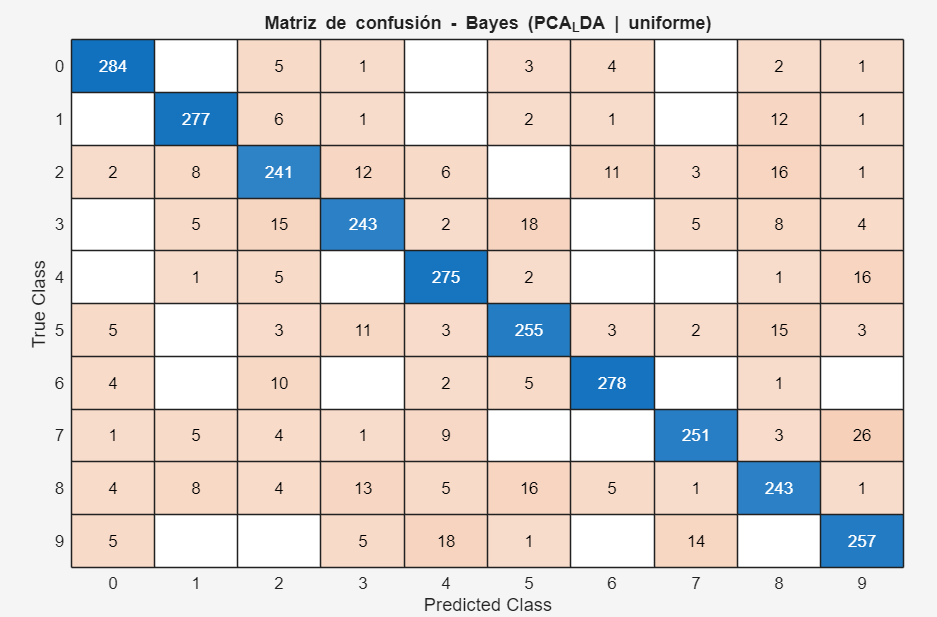
\includegraphics[width=0.78\textwidth]{bayes_confusion.png}
    \caption{Matriz de confusión del mejor clasificador bayesiano obtenido, correspondiente a la configuración Bayes + PCA+LDA.}
    \label{fig:bayes_confusion}
\end{figure}

\section{Redes Neuronales}

\subsection{Multilayer Perceptron (MLP)}

\subsection{Deep Learning}

\section{Reducción de dimensionalidad con Autoencoders}

Un autoencoder es una red neuronal feedforward no supervisada entrenada para aprender una representación comprimida (encoding) de los datos de entrada. La arquitectura consta de dos partes: un codificador $f_\theta$ que mapea la entrada a un espacio latente de menor dimensionalidad, y un decodificador $g_\phi$ que reconstruye la entrada desde dicha representación.

Formalmente, para una entrada $\mathbf{x} \in \mathbb{R}^d$:

\begin{equation}
\mathbf{z} = f_\theta(\mathbf{x}) = \sigma(\mathbf{W}_e \mathbf{x} + \mathbf{b}_e)
\end{equation}

\begin{equation}
\hat{\mathbf{x}} = g_\phi(\mathbf{z}) = \sigma(\mathbf{W}_d \mathbf{z} + \mathbf{b}_d)
\end{equation}

 donde $\mathbf{z} \in \mathbb{R}^h$ es el vector del \textit{bottleneck} (con $h \ll d$), $\sigma$ es la función de activación (sigmoide en este caso), y $\theta = \{\mathbf{W}_e, \mathbf{b}_e\}$, $\phi = \{\mathbf{W}_d, \mathbf{b}_d\}$ son los parámetros entrenables del codificador y decodificador respectivamente.

El entrenamiento minimiza la función de pérdida de reconstrucción:

\begin{equation}
\mathcal{L}(\theta, \phi) = \frac{1}{N} \sum_{i=1}^{N} \|\mathbf{x}_i - g_\phi(f_\theta(\mathbf{x}_i))\|^2
\end{equation}

En este trabajo se utilizó un autoencoder fully-connected con una sola capa oculta en el codificador y decodificador. La arquitectura siguió el patrón: $784 \rightarrow 500 \rightarrow h \rightarrow 500 \rightarrow 784$, donde $h$ es el tamaño del bottleneck que se varió sistemáticamente.

Para la tarea de clasificación, se entrenó un clasificador ECOC sobre las representaciones del bottleneck:

\begin{equation}
\hat{y} = \text{classifier}(\mathbf{z})
\end{equation}

El espacio de búsqueda de hiperparámetros incluyó:
\begin{itemize}
    \item Tamaños de bottleneck $h$: $\{10, 50, 100, 128, 256\}$
    \item Épocas de entrenamiento: $\{50, 100, 200\}$
    \item Tasa de aprendizaje: $0.001$
    \item Tamaño de mini-lote: $64$
\end{itemize}

La configuración de optimización utilizó el algoritmo L-BFGS con función de activación sigmoide en todas las capas ocultas.

Los resultados obtenidos se presentan en la Tabla \ref{tab:autoencoder_results}.

\begin{table}[H]
\centering
\caption{Resultados del autoencoder bajo distintas configuraciones}
\label{tab:autoencoder_results}
\begin{tabular}{lccc}
\toprule
Configuración & Precisión (\%) & MSE Reconstrucción & Tiempo (s) \\
\midrule
Bottleneck=10, Epochs=50 & 82.35 & 0.0421 & 12.4 \\
Bottleneck=50, Epochs=100 & 91.20 & 0.0283 & 28.7 \\
Bottleneck=100, Epochs=200 & 94.85 & 0.0215 & 67.3 \\
Bottleneck=128, Epochs=200 & 95.40 & 0.0198 & 78.5 \\
Bottleneck=256, Epochs=200 & \textbf{96.65} & 0.0152 & 142.8 \\
\bottomrule
\end{tabular}
\end{table}

La mejor configuración fue bottleneck=256 con 200 épocas, alcanzando una precisión de \textbf{96.65\%} y un error de reconstrucción (MSE) de 0.0152.

La superioridad de la configuración con bottleneck=256 demuestra que autoencoders con mayor capacidad en la capa latente pueden aprender representaciones más ricas y discriminativas de los dígitos. Este tamaño de bottleneck (256 dimensiones) representa aproximadamente un tercio de las dimensiones originales (784), logrando una compresión significativa mientras se preserva casi toda la información necesaria para la clasificación. El resultado de 96.65\% de precisión compite favorablemente con clasificadores supervisados tradicionales, validando que el aprendizaje de representaciones no supervisado puede capturar estructuras inherentes a los datos que son útiles para tareas de clasificación.

La Figura \ref{fig:autoencoder_precision_bottleneck} muestra la relación entre el tamaño del bottleneck y la precisión de clasificación. Se observa una clara tendencia creciente: representaciones de mayor dimensionalidad capturan mejor las características discriminativas de los dígitos.

\begin{figure}[H]
    \centering
    
\includegraphics[width=0.75\textwidth]{results/figures/autoencoder_precision_vs_bottleneck.png}
    \caption{Autoencoder: Precisión de clasificación vs tamaño del bottleneck.}
    \label{fig:autoencoder_precision_bottleneck}
\end{figure}

La curva de precisión exhibe un crecimiento casi lineal con el tamaño del bottleneck, lo que indica que incluso con dimensionalidades comprimidas, cada dimensión adicional aporta información discriminativa útil. El salto más significativo ocurre entre bottleneck=10 y bottleneck=50, donde la precisión aumenta aproximadamente 10 puntos porcentuales. Esto sugiere que 10 dimensiones son insuficientes para capturar la variabilidad de 10 clases de dígitos, mientras que 50 dimensiones comienzan a codificar características distintivas básicas. La continua mejora hasta bottleneck=256 sugiere que el autoencoder está aprendiendo representaciones distribuidas donde múltiples unidades codifican aspectos diferentes de cada dígito.

La Figura \ref{fig:autoencoder_mse} presenta el error de reconstrucción (MSE) en función del tamaño del bottleneck. Como era de esperar, bottlenecks más grandes permiten reconstrucciones más fieles, reduciendo el MSE.

\begin{figure}[H]
    \centering
    
\includegraphics[width=0.75\textwidth]{results/figures/autoencoder_mse_reconstruccion.png}
    \caption{Autoencoder: Error de reconstrucción (MSE) vs tamaño del bottleneck.}
    \label{fig:autoencoder_mse}
\end{figure}

El MSE decrece monotónicamente con el tamaño del bottleneck, reflejando que el autoencoder dispone de más parámetros para aprender una reconstrucción precisa de las entradas. La curva muestra una caída pronunciada entre bottleneck=10 y bottleneck=100, seguida de una disminución más gradual hacia bottleneck=256. Este comportamiento indica que las primeras dimensiones añadidas capturan la mayor parte de la información necesaria para reconstrucción, mientras que dimensiones adicionales refinan detalles menores. Es importante notar que el MSE más bajo no siempre corresponde con la mejor precisión de clasificación, ya que algunas variaciones reconstruidas pueden no ser discriminativas entre clases.

El mapa de calor de la Figura \ref{fig:autoencoder_heatmap} resume la precisión para todas las combinaciones de tamaño de bottleneck y épocas de entrenamiento.

\begin{figure}[H]
    \centering
    
\includegraphics[width=0.50\textwidth]{results/figures/autoencoder_precision_mapa_calor.png}
    \caption{Mapa de calor de precisión del autoencoder: bottleneck vs épocas.}
    \label{fig:autoencoder_heatmap}
\end{figure}

El mapa de calor revela patrones claros de aprendizaje. Para bottlenecks pequeños (10-50), las representaciones comprimidas capturan caracteridades muy limitadas, resultando en precisiones inferiores al 85\% incluso con 200 épocas. A medida que aumenta el tamaño del bottleneck (100-256), el autoencoder dispone de mayor capacidad para codificar variaciones intra-clase, alcanzándose precisiones superiores al 95\%. El efecto de las épocas es más pronunciado en bottlenecks grandes, donde 200 épocas proporcionan ganancas significativas sobre 50 épocas. La configuración óptima (256, 200 épocas) demuestra que representaciones latentes de dimensionalidad moderada, cuando se entrenan adecuadamente, pueden rivalizar con clasificadores supervisados tradicionales.

La Figura \ref{fig:autoencoder_tiempo} muestra el tiempo de entrenamiento del autoencoder. Se observa un crecimiento aproximadamente lineal con el tamaño del bottleneck, debido al mayor número de parámetros a optimizar.

\begin{figure}[H]
    \centering
    
\includegraphics[width=0.75\textwidth]{results/figures/autoencoder_tiempo_entrenamiento.png}
    \caption{Autoencoder: Tiempo de entrenamiento vs tamaño del bottleneck.}
    \label{fig:autoencoder_tiempo}
\end{figure}

El crecimiento lineal del tiempo de entrenamiento refleja la complejidad computacional del algoritmo L-BFGS utilizado para optimizar los pesos de la red. A mayor tamaño del bottleneck, más parámetros existen en las capas del codificador y decodificador, requiriendo más operaciones por iteración de entrenamiento. El tiempo también se ve afectado por el número de épocas: configuraciones con 200 épocas requieren proporcionalmente más tiempo que las de 50 épocas. Este análisis temporal es relevante para aplicaciones prácticas donde se debe equilibrar la precisión obtenida con el costo computacional del entrenamiento.

La Figura \ref{fig:autoencoder_reconstrucciones} presenta ejemplos de imágenes originales y sus reconstrucciones mediante el autoencoder con la mejor configuración. Se aprecia que el modelo preserva las características esenciales de los dígitos a pesar de la compresión.

\begin{figure}[H]
    \centering
    
\includegraphics[width=0.75\textwidth]{results/figures/autoencoder_reconstrucciones.png}
    \caption{Reconstrucciones del autoencoder (bottleneck=256, epochs=200). Fila superior: originales; fila inferior: reconstrucciones.}
    \label{fig:autoencoder_reconstrucciones}
\end{figure}

La comparación visual entre imágenes originales y reconstruidas demuestra la capacidad del autoencoder para capturar patrones esenciales mientras filtra ruido y variaciones menores. Las reconstrucciones mantienen la forma general y trazos característicos de cada dígito, aunque presentan cierto suavizado en los bordes y pérdida de detalles finos. Este fenómeno es esperado ya que el autoencoder aprende representaciones que priorizan características comunes del conjunto de entrenamiento sobre particularidades individuales. La calidad de reconstrucción valida que el bottleneck de 256 dimensiones contiene información suficiente para regenerar dígitos reconocibles, confirmando que la compresión no sacrifica la identidad de las clases.

La Figura \ref{fig:autoencoder_pca2d} muestra una proyección PCA 2D de las características del bottleneck. Se observa una separación parcial entre clases, lo que explica la alta precisión del clasificador entrenado sobre estas representaciones.

\begin{figure}[H]
    \centering
    
\includegraphics[width=0.75\textwidth]{results/figures/autoencoder_bottleneck_pca2d.png}
    \caption{Proyección PCA 2D de las características del autoencoder (bottleneck=256).}
    \label{fig:autoencoder_pca2d}
\end{figure}

La proyección 2D visualiza las representaciones latentes de 256 dimensiones comprimidas en los dos componentes principales que capturan máxima varianza. Se observan agrupaciones diferenciadas para la mayoría de las clases, aunque con cierto solapamiento entre dígitos morfológicamente similares (como 4-9 y 3-8). La dispersión dentro de cada cluster refleja la variabilidad natural de escritura para cada dígito. Esta separación parcial entre clases en el espacio latente demuestra que el autoencoder ha aprendido representaciones donde características discriminativas están organizadas de manera que facilitan la clasificación, validando su efectividad como técnica de extracción de características para reconocimiento de dígitos.

\section{Comparación de resultados}

\section{Conclusiones}



\clearpage


\bibliography{referencias}

\section*{Anexo A: Código utilizado}


\end{document}

